%*****start of file apssamp.tex ******
%
%   This file is part of the APS files in the REVTeX 4.1 distribution.
%   Version 4.1r of REVTeX, August 2010
%
%   Copyright (c) 2009, 2010 The American Physical Society.
%
%   See the REVTeX 4 README file for restrictions and more information.
%
% TeX'ing this file requires that you have AMS-LaTeX 2.0 installed
% as well as the rest of the prerequisites for REVTeX 4.1
%
% See the REVTeX 4 README file
% It also requires running BibTeX. The commands are as follows:
%
%  1)  latex apssamp.tex
%  2)  bibtex apssamp
%  3)  latex apssamp.tex
%  4)  latex apssamp.tex
%
\documentclass[aps,prl,twocolumn,showpacs,floatfix,superscriptaddress]{revtex4-1}
\usepackage{dcolumn}
\usepackage{bm}

\usepackage{soul}
\usepackage{amsmath,amssymb,graphicx}
\usepackage[colorlinks=true,citecolor=blue,urlcolor=blue,linkcolor=blue]{hyperref}

\bibliographystyle{apsrev4-1}
%\documentclass[%
 %reprint,
%superscriptaddress,
%groupedaddress,
%unsortedaddress,
%runinaddress,
%frontmatterverbose, 
%preprint,
%showpacs,preprintnumbers,
%nofootinbib,
%nobibnotes,
%dsbibnotes,
% amsmath,amssymb,
 %aps,
%pra,
%prb,
%rmp,
%prstab,
%prstper,
%floatfix,
%]{revtex4-1}

%\usepackage{graphicx}% Include figure files
%\usepackage{dcolumn}% Align table columns on decimal point
%\usepackage{bm}% bold math
%\usepackage{hyperref}% add hypertext capabilities
%\usepackage[mathlines]{lineno}% Enable numbering of text and display math
%\linenumbers\relax % Commence numbering lines

%\usepackage[showframe,%Uncomment any one of the following lines to test 
%%scale=0.7, marginratio={1:1, 2:3}, ignoreall,% default settings
%%text={7in,10in},centering,
%%margin=1.5in,
%%total={6.5in,8.75in}, top=1.2in, left=0.9in, includefoot,
%%height=10in,a5paper,hmargin={3cm,0.8in},
%]{geometry}
\usepackage{subfig}
\DeclareGraphicsExtensions{.png,.jpg,.pdf}
%\DeclareGraphicsExtensions{.pdf,.png,.jpg}
\graphicspath{{../figures/}} % Directory in which figures are stored
%\usepackage[square,numbers]{natbib}
%\bibliographystyle{abbrvnat}
\begin{document}

%\preprint{APS/123-QED}

\title{Dynamical Mean Field Theory of Strongly Correlated Electrons in 2D}% Force line breaks with \\
%\thanks{A footnote to the article title}%

\author{Omadillo Abdurazakov}
% \email{oabdura@ncsu.edu}
% \altaffiliation[Also at ]{Department of Physics, NC State University.}%Lines break automatically or can be forced with \\
% \email{akemper@ncsu.edu}
\affiliation{%
Department of Physics, NC State University, Raleigh, NC, 27695, USA
}%

%\collaboration{MUSO Collaboration}%\noaffiliation

%\author{Charlie Author}
% \homepage{http://www.Second.institution.edu/~Charlie.Author}
%\affiliation{
% Second institution and/or address\\
% This line break forced% with \\
%}%
%\affiliation{
% Third institution, the second for Charlie Author
%}%
%\author{Delta Author}
%\affiliation{%
% Authors' institution and/or address\\
% This line break forced with \textbackslash\textbackslash
%}%

%\collaboration{CLEO Collaboration}%\noaffiliation

%\date{}% It is always \today, today,
             %  but any date may be explicitly specified

\begin{abstract}
We study the behaviour of the strongly interacting electrons in a two dimensional tight binding band at half filling by solving the Dynamical Mean Field Theory(DMFT) equations. Through the calculation of the density of states at different temperatures and the electron-electron interaction strengths we find a metal-insulator transition around 4.0 eV. We also observe that whether the sytem is metallic or insulating is a result of the interplay between interaction strength and temperature. 
\end{abstract}

%\pacs{Valid PACS appear here}% PACS, the Physics and Astronomy
                             % Classification Scheme.
%\keywords{Suggested keywords}%Use showkeys class option if keyword
                              %display desired
\maketitle

%\tableofcontents

\section{\label{sec:intro}Introduction}
The strong electron-electron correlations, although complicates the problem at hand, enriches the physics of many-body system with veriety of phenonmena like high-temperature superconductivy, Mott metal-insulator transition, itenarant ferromagnitism and so on\cite{georges}. The Hubbard model of interacting electrons is one of the most used models to study these phenomena. Many methods have been developed to solve this model. The Dynamical Mean Field Theory (DMFT) and its hybrid versions combined with different numerical techniques have been successful in this mattter\cite{georges}. Here we use the Iterative Perturbation scheme to solve the DMFT equations for the Hubbard model. 
\section{\label{sec:method}Model and Method}
Here  we consider following Hubbard Hamiltonian
\begin{eqnarray}
        \mathcal{H} =  \sum_{\textbf{k}\sigma} \epsilon_{\textbf{k}}c_{\textbf{k},\sigma}^{\dagger}
        c_{\textbf{k},\sigma} + U \sum_i n_{i\uparrow}n_{i\downarrow},
\end{eqnarray}
discribing the electrons with on-site interaction $U$ and residing in a single tight-binding band depicted in FIG.~\ref{fig:1} and given by 
\begin{eqnarray}
        \epsilon_{\textbf{k} } = -2t(cosk_x + cosk_y),
\end{eqnarray}
where they can hop between adjacent sites with an amplitude of $t$. Here $c_{\textbf{k},\sigma}$ and $c_{\textbf{k},\sigma}^{\dagger}$ are the electronic annihilation and creation field operators in the state $\textbf{k}$ with the spin $\sigma$, while $n_i = c_i^\dagger c_i$.
	\begin{figure}
		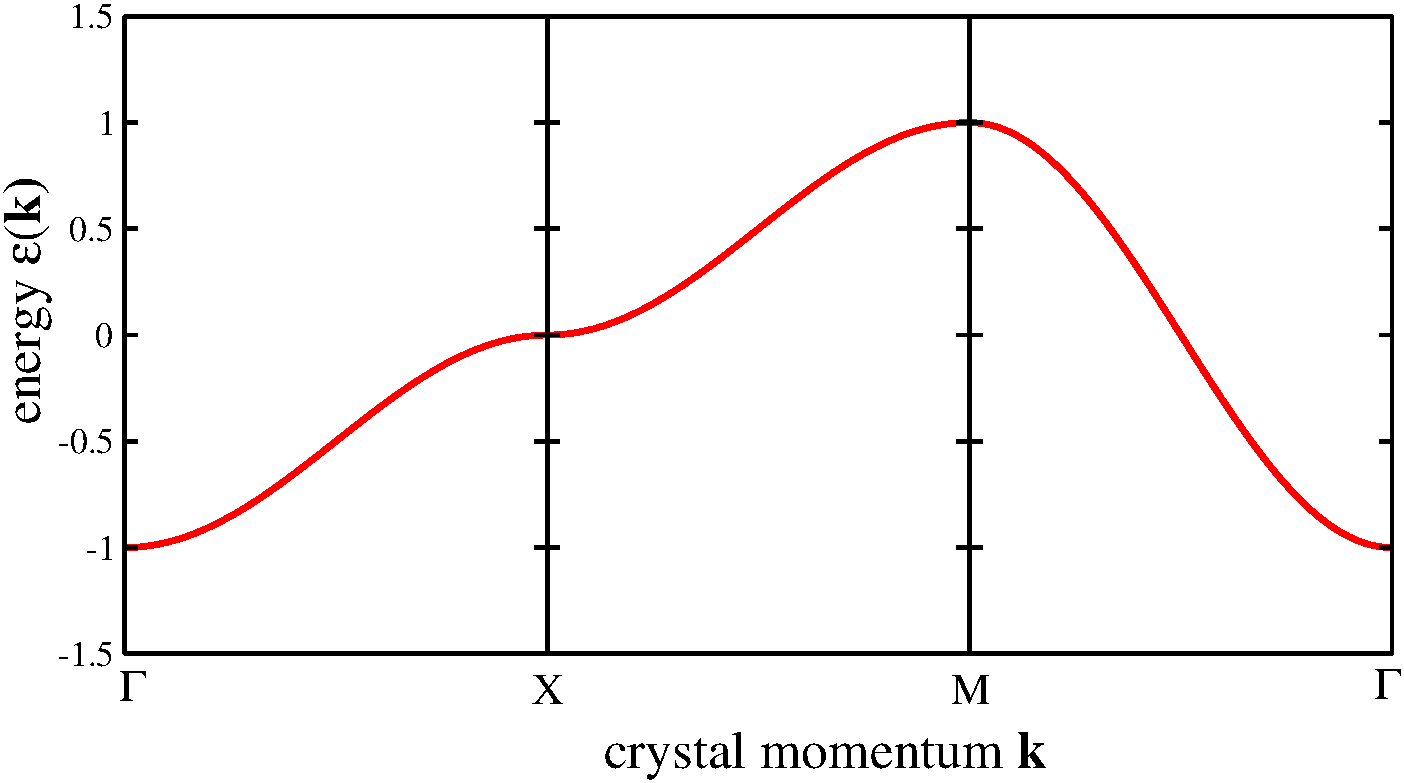
\includegraphics[scale=0.3,angle=0]{band}
		\caption{The electronic band structure plotted through the high symmetry momentum points}
		\label{fig:1}
	\end{figure}


On of the early and successful methods to solve the problem in the framework of DMFT was through the Iterative Perturbation(IP) theory approximation\cite{georges92}. It gives a qualitative explanation of Mott metal-insulator transition and easily solved iteratively. Here we use this method for our half-filled single band Hubbard model. The first order terms in the perturbative expansion can be absorbed into the chemical potential which we take to be zero\cite{georges}, so we can treat the self-energy in the second order.
In the infinite special dimension, the self-energy becomes momentum independent.
For the 2D density of states
\begin{align}
D(\omega) =& \sum_{\textbf{k}}\delta(\omega - \epsilon_{\textbf k})\nonumber\\ 
	  =& \int \frac{d^2 k}{(2\pi)^2}\int dx e^{-ix(\omega -\epsilon_{\textbf{k}})}\nonumber \\
	  =& \int dx e^{-i\omega x}\int \frac{dk_x}{2\pi}e^{2txcosk_x}\int \frac{dk_y}{2\pi}e^{2txcosk_y}\nonumber\\
	  =& \int dx e^{-i\omega x}J_0^2(2t x)\nonumber \\
	  =& \int_0^{\infty} dx cos(\omega x)J_0^2(2t x)\nonumber\\
\end{align}

As the dimention gets higher the DOS converges to a normal distribution at $d = \infty$. However, we can see from FIG.\ref{fig:3} that the shape of DOS at $d = 8$ resembles that of the inifinite dimension. Therefore, approximating the self-energy to be local in space gives some qualitatively good results even for small dimenstions. And the self-energy becomes a functional of the local Green's function which is equal to the impurity Green's function at high dimensions. 
\begin{align}
G_{imp}(\omega) = G_{loc}(\omega) = \sum_{\textbf k}\frac{1}{\omega - \epsilon_{\textbf k}- \Sigma_{imp}}
\end{align}

The single-particle self-energy of 2nd order in $U$ depicted pictorially in the FIG.~\ref{fig:2} represents the following expression.
\begin{align}
\Sigma_{\textbf k}(ik_n) =& -{U^2 T^2}\sum_{\textbf{k}',\textbf{q},ik_n,iq_n}G_{\textbf{k}'}(ik'_n)G_{\textbf{k}'-\textbf{q}}(ik'_n-iq_n)\nonumber\\
&\times G_{\textbf{k}-\textbf{q}}(ik_n-iq_n)
\end{align}
	\begin{figure}
		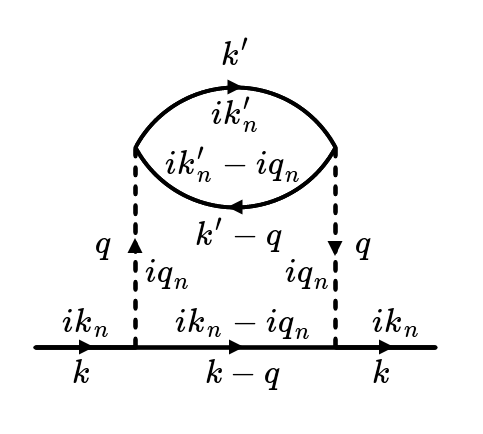
\includegraphics[scale=0.3,angle=0]{matsubara}
		\caption{The second order self-energy diagram in frequency domain}
		\label{fig:2}
	\end{figure}

As the main approximation of DMFT is the local nature of the self-energy at high dimensions, we can rewrite it as
\begin{align}
\Sigma_{imp}(ik_n) =& -{U^2 T^2}\sum_{ik_n,iq_n}G(ik'_n)G(ik'_n-iq_n)\nonumber\\
&\times G(ik_n-iq_n)\\
=&-U^2 T^2 \sum_{iq_n}\Pi(iq_n)\int \frac{dx}{\pi}\frac{ImG(x)}{x-ik_n-iq_n},
\end{align}
where the polarization function is 
\begin{align}
\Pi(iq_n) = - \int \frac{dx}{\pi}ImG(x)n_F(x)[G(x+iq_n) + G(x - iq_n)].
\end{align}
After a short manipulation and analytic continuation to the real axis $ik_n \rightarrow \omega + i\delta$, for the imaginary part of the self-energy we arrive at

\begin{align}
Im \Sigma(\omega) = &  U^2\int dx Im G(\omega-x)n_F(\omega-x)\nonumber\\
\times & \int dy ImG(x)n_F(x)ImG(x-y)(1-n_F(x-y))\nonumber\nonumber\\
+& U^2\int dx Im G(\omega-x)(1-n_F(\omega-x))\nonumber\\
\times & \int dy ImG(x)n_F(x)ImG(y-x)(1-n_F(x))) 
\end{align}
The the real part of the self-energy can be computed through the Kramers-Kronig relationship
\begin{align}
Re\Sigma(\omega)=&\frac{1}{\pi}\mathcal{P}\int dx\frac{Im\Sigma(x)}{x-\omega}.
\end{align}
Through the Dyson equation new impurity Green's function can be recomputed as
\begin{align}
G_0(\omega) = \frac{1}{G(\omega)^{-1}+\Sigma(\omega)},
\end{align}
which can be used to calculate the new self-energy and repeat the iteration until the convergence is achieved when the impurity Green's function and self-energy are equal to those of the lattice.

	\begin{figure}
		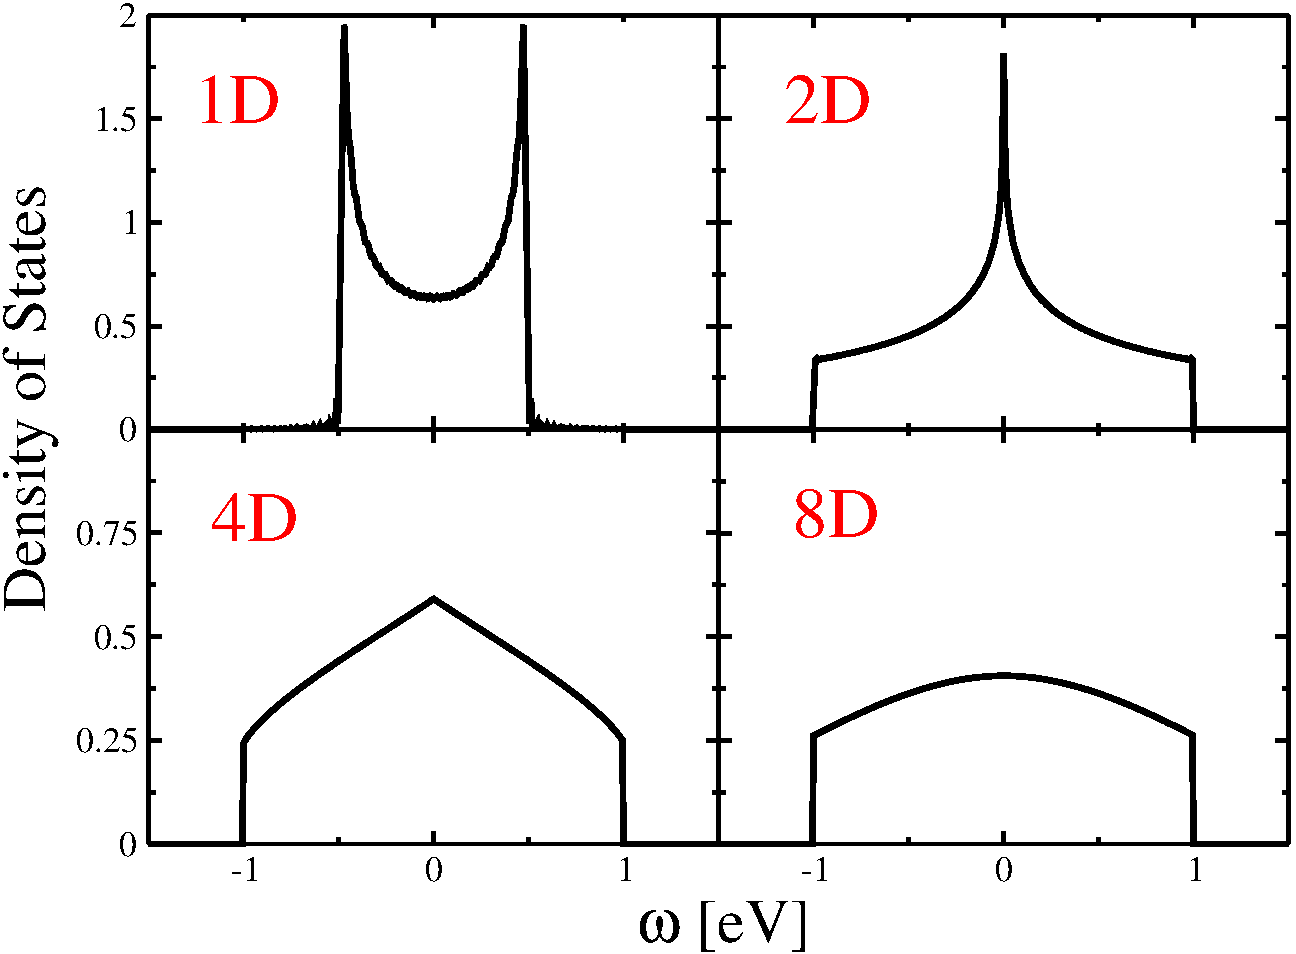
\includegraphics[scale=0.3,angle=0]{densities}
		\caption{The density of states at different special dimensions in an increasing order}
		\label{fig:3}
	\end{figure}

\section{\label{sec:method}Results}
As thermodynamic, optical, and electrical properties of strongly correlated materials are highly dependent upon the density of states around the Fermi level $DOS(\omega = \epsilon_F)$, we have studied $DOS(\omega) = -\frac{1}{\pi}G_{loc}(\omega)$ at different interaction streangths $U$ and temperatures $T$. In FIG.\ref{fig:1} we compare the bare density of states with those of different $U$s at $T = 0.02 eV$.At the values of $U < 4.5 eV$ we a metallic state with three distinct peaks.  In addition to the so-called Abrikosov-Suhl resononant quasiparticle peak at $\epsilon_F$, the bare band split into the lower and upper Hubbard bands. The quasiparticle peak weight is renormalized by $Z = -\frac{\partial Re\Sigma(\omega)}{\partial \omega}$  at $\omega = 0$ \cite{muller}.  The larger $U$ makes the system a bad metal. When the magnitude of $U$ reaches around $4.5 eV$ the system a Mott metal-insulating transition takes place. Here the two split bands are located at approximately $\pm\frac{U}{2}$ under the electron-electron interaction. If the half-filled bare band have a single electron per site, the lower band is full and upper is empty. We also study the behaviour of the insulating phase as a function of temperature in FIG.\ref{fig:5}. As expected the solution becomes aa bad insulator as the temperature is raised. After $T = 0.03 eV$ the we start restoring the metallic state. In addition, we also study the changes in the metallic phase as the temperature is changed in FIG.\ref{fig:6}. It is counter-intuitive to see that the system becomes a slightly better metal as the temperature is increased.


	\begin{figure}
		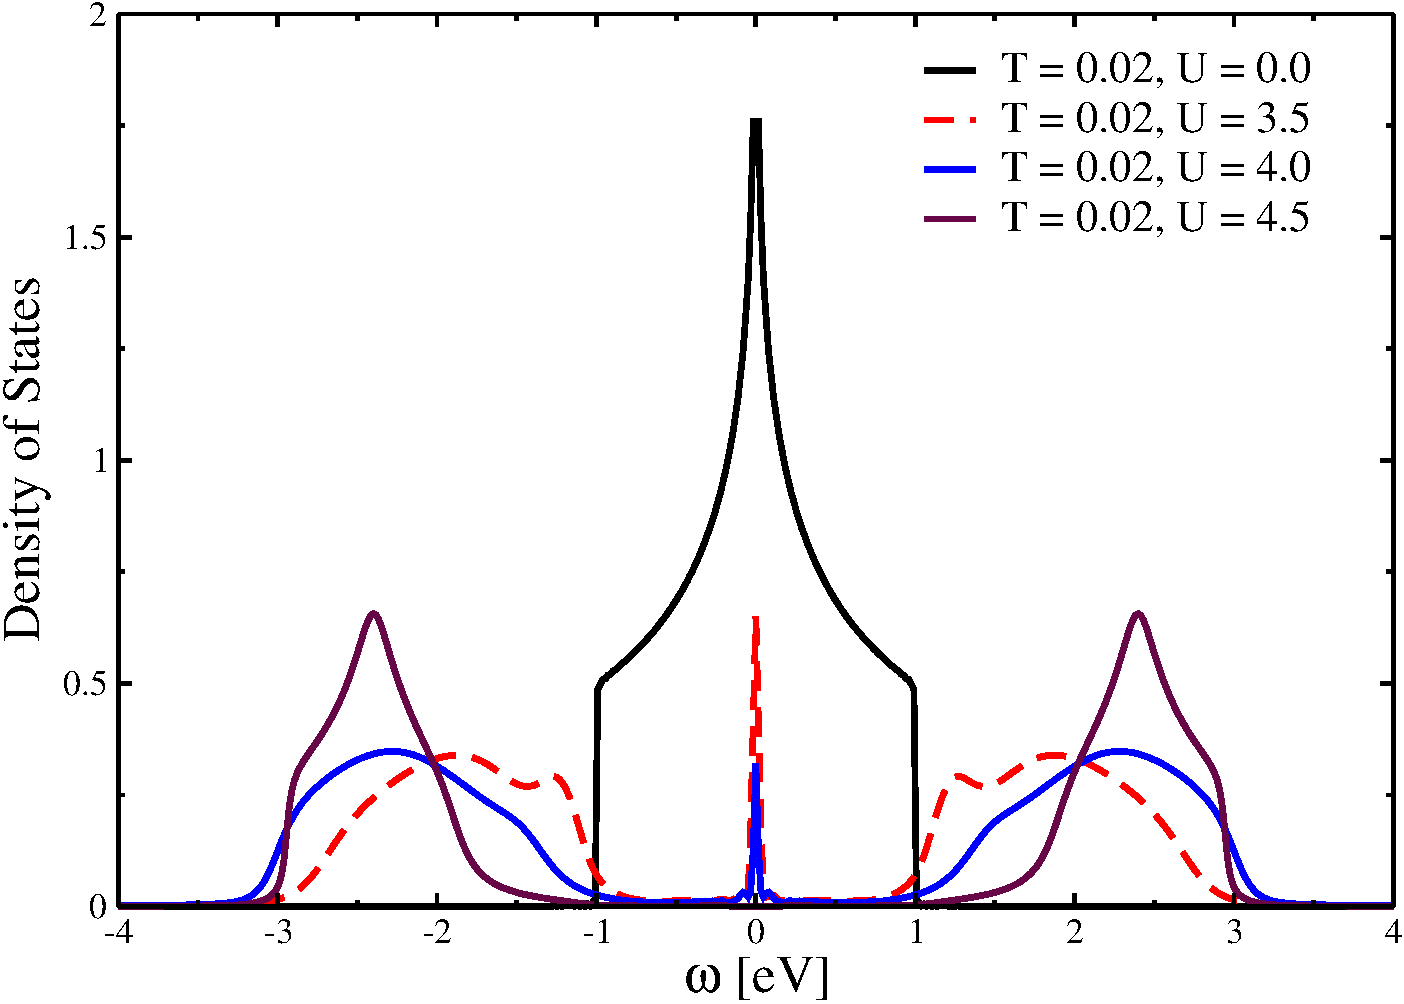
\includegraphics[scale=0.3,angle=0]{u}
		\caption{The Mott metal-insulating transition}
		\label{fig:4}
	\end{figure}

	\begin{figure}
		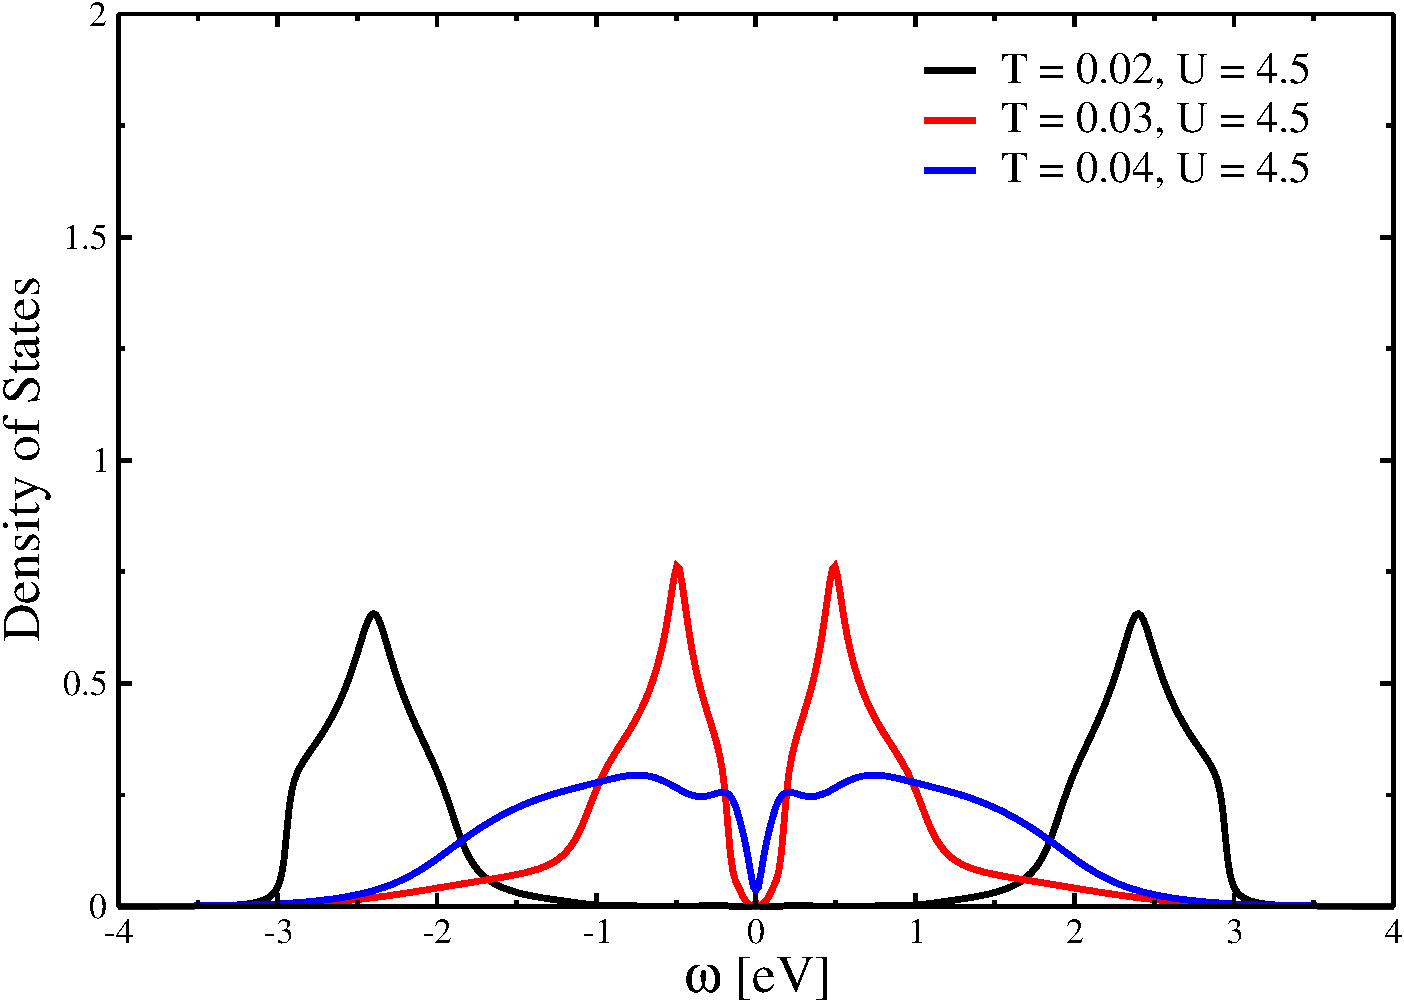
\includegraphics[scale=0.3,angle=0]{tempins}
		\caption{The effect of temperature on the insulating state}
		\label{fig:5}
	\end{figure}
	
	\begin{figure}
		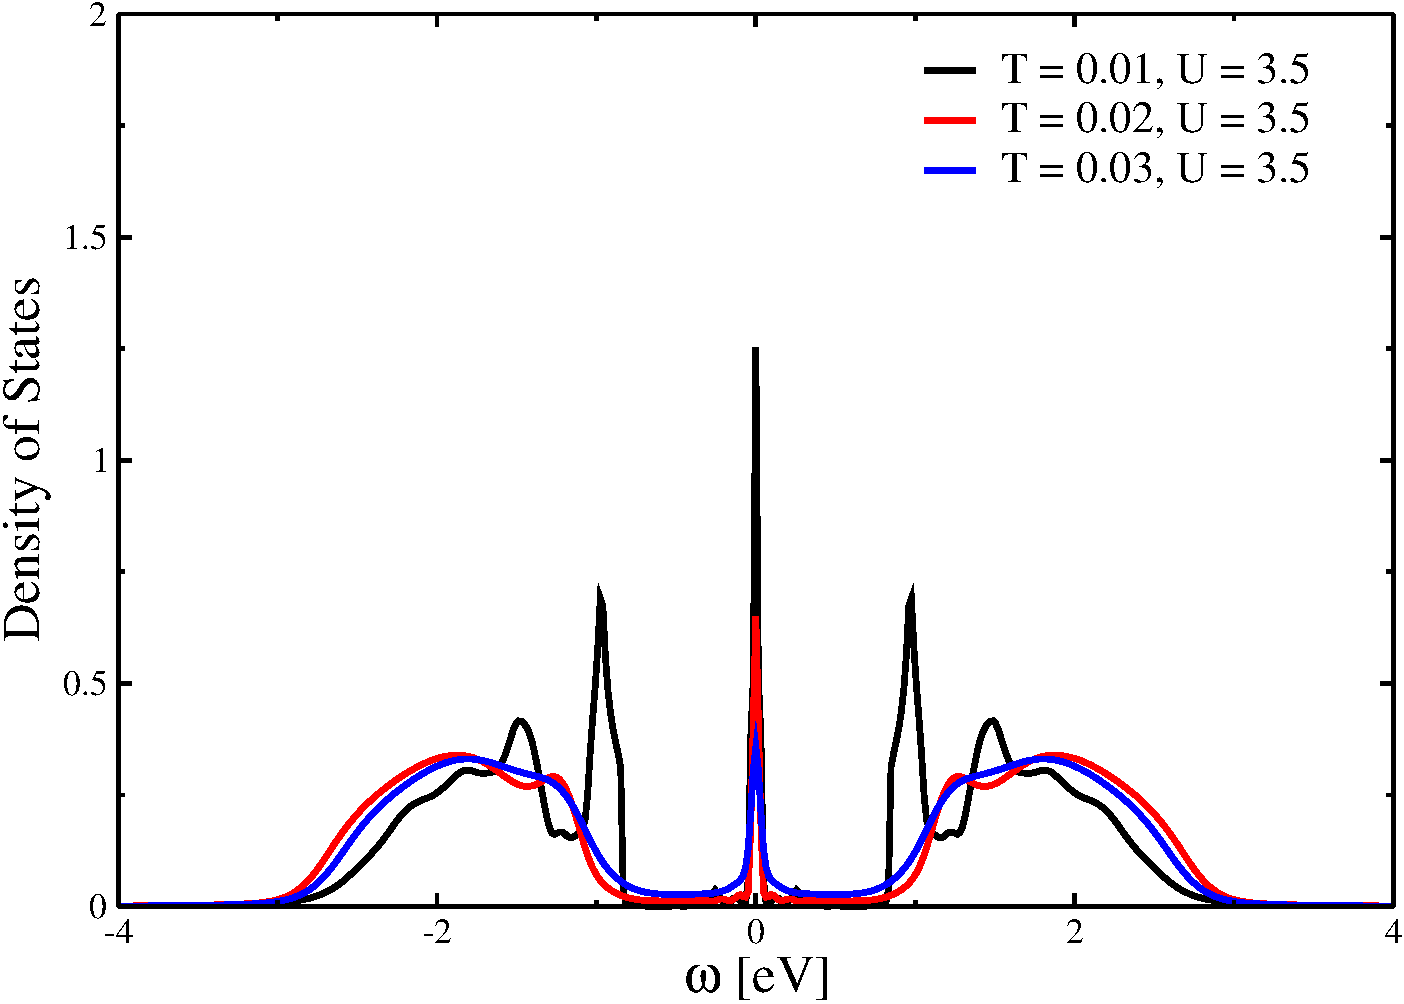
\includegraphics[scale=0.3,angle=0]{tempmetal}
		\caption{The effect of temperature on the metallic state}
		\label{fig:6}
	\end{figure}
%\section{\label{sec:discussion}Discussion}

\section{\label{sec:conclusion}Conclussion}
As we have shown that the Hubbard Hamiltonian solved through the Iterative Perturbation method in the framework of DMFT gives a simple qualitative descrtiption of the strongly correlated systems. The competition between the kinetic and the interaction terms in the Hamiltonian causes the system to take either a metallic or an insulating phase. Through solving the DMFT self-consistent equations the Mott transiton can be obtained.
\begin{thebibliography}{1}
        \bibitem{georges} A. Georges, G. Kotliar, W. Krauth, and M. J. Rezenberg, Rev.Mod.Phys. \textbf{68}, 13 (1996)
	\bibitem{metzner} W. Metzner and D. Vollhardt, Phys. Rev. Lett. \textbf{62}, 324(1989)
	\bibitem{georges92} A. Georges, and G. Kotliar, Phys. Rev. B \textbf{45}, 6479(1992)
	\bibitem{notes} The used algorith closely follows the notes by Kristjan Haule url: thttp://www.physics.rutgers.edu/~haule/index.html
	\bibitem{eckstein} M. Eckstein, M. Kollar, K. Byczuk and D. Vollhardt, Phys. Rev. B \textbf{71}, 235119(2005)
	\bibitem{muller} E. Muller-Hartmann, Z. Phys. B \textbf{74}, 507 (1989)
\end{thebibliography}

\end{document}
%
% ****** End of file apssamp.tex ******

